% Chapter 4

\chapter{Instrumentation: Gradient elution SFC} % Write in your own chapter title
\label{Chapter4}
\lhead{Chapter 4. \emph{Gradient SFC}} % Write in your own chapter title to set the page header

\section{Supercritical Fluid Chromatography}

The source of high-pressure carbon dioxide for SFC was high-purity carbon dioxide from Air Products. Carbon Dioxide 4.5, meaning carbon dioxide that is 99.995\% pure. 

At 5.6 MPa the pressure is not near the supercritical range. It is a mere 55.3 atm, while we do the supercritical chromatography at 200 atm. The critical pressure of carbon dioxide is 7.39 MPa. At 200 atm, which translates to 20.27 MPa, there is 

We work at below the critical temperature of carbon dioxide, (an easy-to-remember 300K, or 37�C), but by using such a high pressure it means that the gas is overwhelmingly in the liquid phase.

(It is widely recognized in the field now that SFC has become a misnomer. SCF is not usually done above the critical temperature, and sometimes at quite modest pressures. At Pittcon 2010 I heard someone refer to it as `Separation Facilitated by Carbon dioxide'.)

\begin{figure}[htbp]
	\centering
	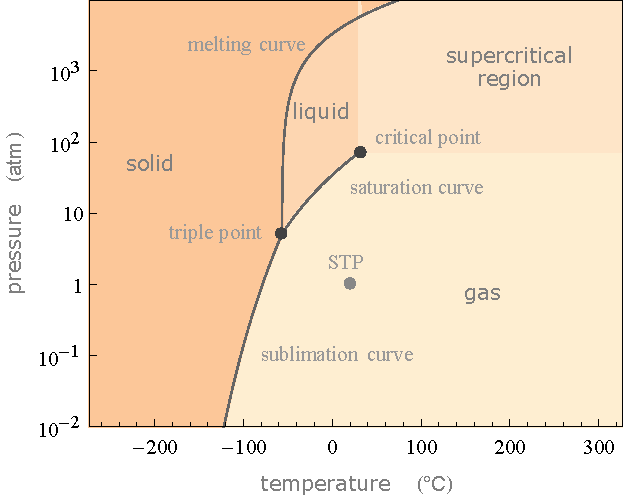
\includegraphics[width=0.8\textwidth,natwidth=4.17in,natheight=3.32in]{./Figures/CO2pVdiagram.pdf}
	\rule{35em}{0.5pt}
	\caption[Phase diagram]{The phase diagram for carbon dioxide}
	\label{fig:PhaseDiagram}
\end{figure}

\section{SFC}
%Varian 8500 LC pump.
%Pressure guage

The liquid carbon dioxide from the cylinder was conducted to the Varian 8500 LC pump.

Although the pump's `Fill' was used to fill the empty cylinder, this should not create the impression that the pump aspirates the liquid carbon dioxide from the bottle. The moment the carbon dioxide enters the pump cylinder, the vapour pressure will be determined by the temperature. While the pump can produce a small amount of underpressure, the vapour pressure will dominate. Therefore a hot pump cylinder will not fill with liquid, because the pressure inside the cylinder will press any liquid back into the dip tube, and the pump will only fill with vapour. The pump needs to be cooled to allow the liquid into the cylinder. 

At 200 atm the pump leaks at xxx nl/s

A chiller from Labotec with a 20 l capacity was filled with a solution of 7.5 l of diethyl glycerol and 7.5 l of water. This mixture has a freezing point of -10 deg C, which can be cooled by the chiller without freezing. (If the coolant freezes a hump of ice forms on the cooling plate of the chiller, which isolates the remaining liquid and limits the temperature of the coolant to the melting point of the coolant.)

Unfortunately the higher viscosity of the mixture compared to water makes it more difficult to pump reducing the pump `head' of the Labotec stirrer/heater/pump so much that it couldn't pump the liquid from the chiller on the floor to the top of the pump cylinder, preventing the circulation of coolant. Therefore an inexpensive submersible WH1200 water pump from Waterhouse was acquired, which can deliver 800 l of water per hour at a head of 1.2m.

We also used a SFT-10 pump from Supercritical Fluid Technologies (Newark, Delaware). This is a purpose-built two-piston pump with a sapphire pistons and a Peltier-cooled head. This is a much better technology than the HPLC pumps. It takes up less space and does not need refilling, since it feeds directly from the cylinder. 

\section{Gradient Elution SFC}

\subsection{Pressure Programming}

In the early days of SFC the solubility of the mobile phase was tuned by adjusting the pressure. Using this adjustability one could obtain gradient elutions by simply adjusting the pressure of the mobile phase.

\subsection{Modifier Programming}
It was soon realized that this tuning range is not particularly wide, and pretty soon people were adding modifiers to the carbon dioxide. Adding a modifier makes dramatic differences to the dissolving power of the carbon dioxide, but reduces the compressibility. This means that varying modifier concentration has replaced pressure tuning as the primary means of gradient elution in SFC. 

We made provision for addition of a single modifier to the carbon dioxide. The SFC system operated under constant pressure, but it was easy to calculate the flow provided by counting the number of steps given by the stepper motor of the pump to maintain that pressure. Before the column we had a six-port valve configured with a injector loop. This loop was filled with methanol from a second HPLC syringe pump. The volume of this loop was determined colourimetrically. By regularly switching the modifier valve the contents of the injection loop is placed in the mobile phase and the selected concentration achieved.

This approach is not without its problems. When the valve switches from ``Inject'' back to ``Load'', the liquid carbon dioxide in the injection loop is exposed to the atmosphere and it expands explosively. Rather unexpectedly, it expands into the methanol supply line, blowing a part of the methanol in it out. (A tentative explanation for this that the high pressure gradient drives bubbles of carbon dioxide gas into the supply tube. As these bubbles expand when the pressure drops, it forces the methanol from the tube.) This emptying of the methanol tube means that the methanol consumption is much higher than one would expect. In the case of using toxic or irritant modifiers one would need a means of extracting the vapours.

Care has to be taken to ensure that the mixing downstream of the valve is adequate, otherwise an oscillating modifier concentration will be result.

%graph of measurement of loop volume?

\subsection{Additive Programming}

Additives are minor compounds that are added to the mobile phase to 

\section{Restrictors}

In HPLC and UPLC, the most common detectors are UV detectors that use pressurized flow cells. After the detector there is a back-pressure controller that controls the pressure in the chromatographic system.

\begin{quote}
Changes in pressure can greatly vary the characteristics of SFC. Achieving extraction and chromatograms with high reproducibility on a supercritical fluid system requires a device that can perform pressure control in a stable manner. JASCO offers the BP-2080, which is capable of automatic pressure control, and the BP-2080-M, which is capable of manual pressure control.
BP-2080/2080-M Back Pressure Regulator

The BP-2080 and BP-2080-M employ a patented flow-switching valve (FSV) mechanism that enables stable system pressure control even at the lowest volume limit possible. The FSV mechanism regulates pressure by controlling the channel opening while a needle vibrates at a high rate of speed. This prevents blockages due to high-viscosity elution samples and solidified samples, which can be a problem with static pressure regulators. This enables stable system pressure, even during long-term continuous operation. Since the BP-2080 has a time program feature that can control pressure and temperature according to the passage of time, it makes it easy to automate analysis work. The BP-2080M offers manual control for the volume passing through the opening in the FSV mechanism.

\end{quote}

In the case of restrictors there is too little we can do.

The restrictor has a two-fold function. \begin{enumerate}
	\item It controls the flow of the eluent from the column. If there is no flow, the pressure difference over the column is zero, and there is no flow. By opening an orifice in the form of a restrictor, there is a flow of eluent from the column, reducing the outlet pressure, thus allowing flow through the column. The size of the orifice controls the pressure at the column outlet, and thereby the chromatographic flow. 
	\item It maintains the pressure inside the chromatographic column at supercritical pressure. 
\end{enumerate}

The restrictor can be of different designs. 

As a first approximation we can use the Hagen-Poiseuille equation

\begin{equation}
Q = \frac{\pi R^4}{8\mu}\frac{\Delta p}{L} 
\label{eqn:Hagen-Poiseuille}
\end{equation}

This is of course only a very rough approxmation, because we are using a compressible, condensing fluid with the temperature dropping quickly because of adiabati expansion. But it will serve to illustrate different approaches.

The linear restrictor uses the pressure drop over the lenght of a straight piece of capillary. This increases $L$, which, for a given length. 

With the integral, or micro-hole, restrictor, the radius of a short length of pipe is controlled. Because of the fourth power, a small increase in radius allows a much greater pressure drop.

The third design, the frit restrictor, uses a combination of small holes and length. The length is the controlled factor.

\begin{description}
	\item[Linear restrictor] The linear restrictor is merely a long piece of 
	\item[Orifice restrictor]
	\item[Frit restrictor] D
\end{description}

We used the `integral' restrictor as described by Guthrie and Schwartz. We've had good experience with these models. It uses only a small amount of capillary column, and gives a good degree of adjustibility, for a fairly simple procedure. The percieved benefit of this design was that it would not cause discrimination by the lenghty pressure drop. 

But in practice we discovered that micro-orifice restrictors blocked. At first it was assumed that it was particles from the stop-flow valve that were blocking the orifice, and we installed a half-micron filter. (Univerversal Mini Filter, 0.5 $\mu$m, Grace, Deerfield Illionois. The restrictor plugging was unpredictable and irregular. To determine the cause of the plugging, , a number of plugged restrictors were prepared for scanning electron microscopy (SEM). 

In many cases there were no plugging visible, but the restrictor still stopped flow. 

To from an idea of what to expect we first examined a blank piece of capillary. 

\begin{figure}[htbp]
	\centering
	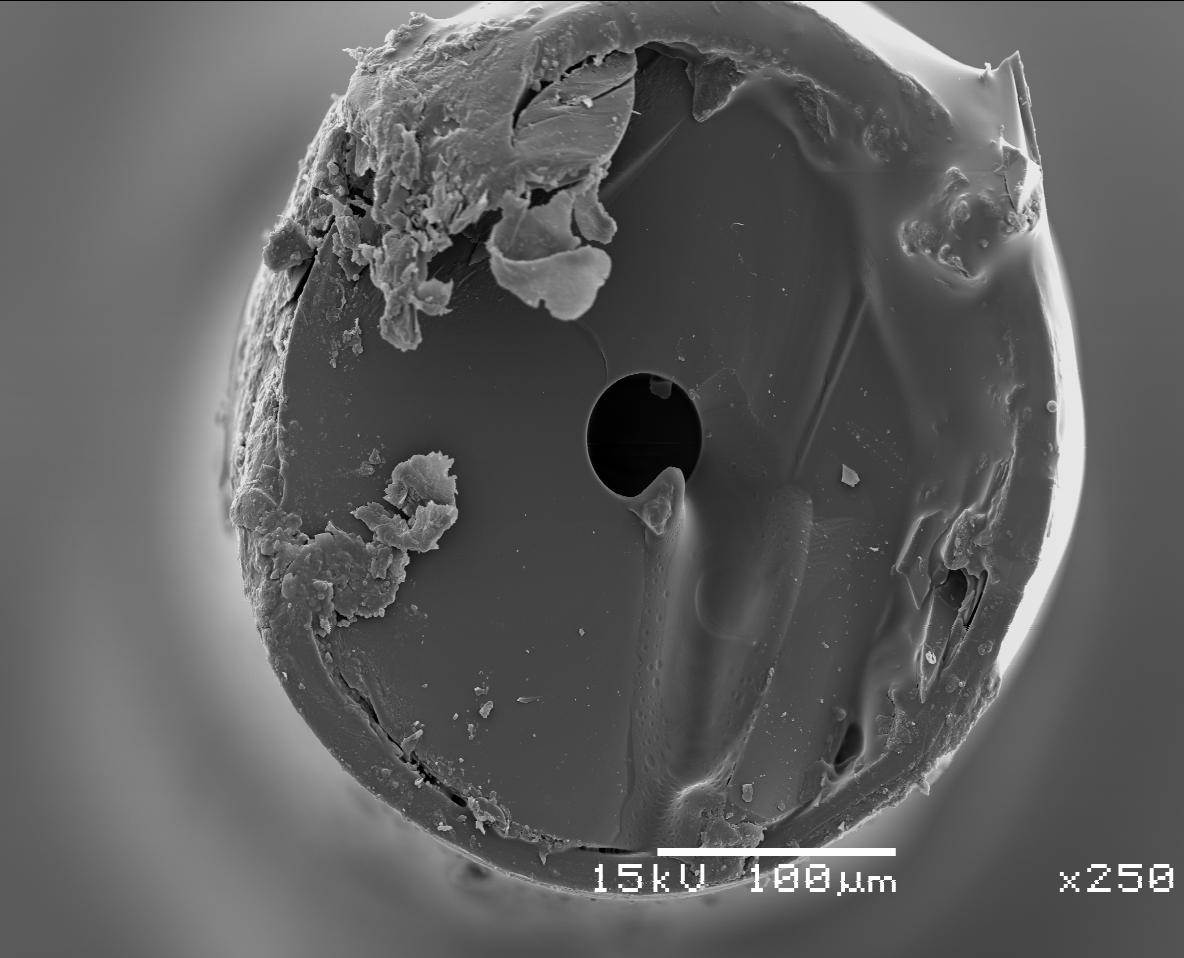
\includegraphics[width=0.8\textwidth,natwidth=4.17in,natheight=3.32in]{./Figures/A_001.pdf}
	\rule{35em}{0.5pt}
	\caption["SEM image of a capillary end."]{"A SEM image of a capillary end."}
	\label{fig:A001}
\end{figure}

A close-up image of the 

\begin{figure}[htbp]
	\centering
	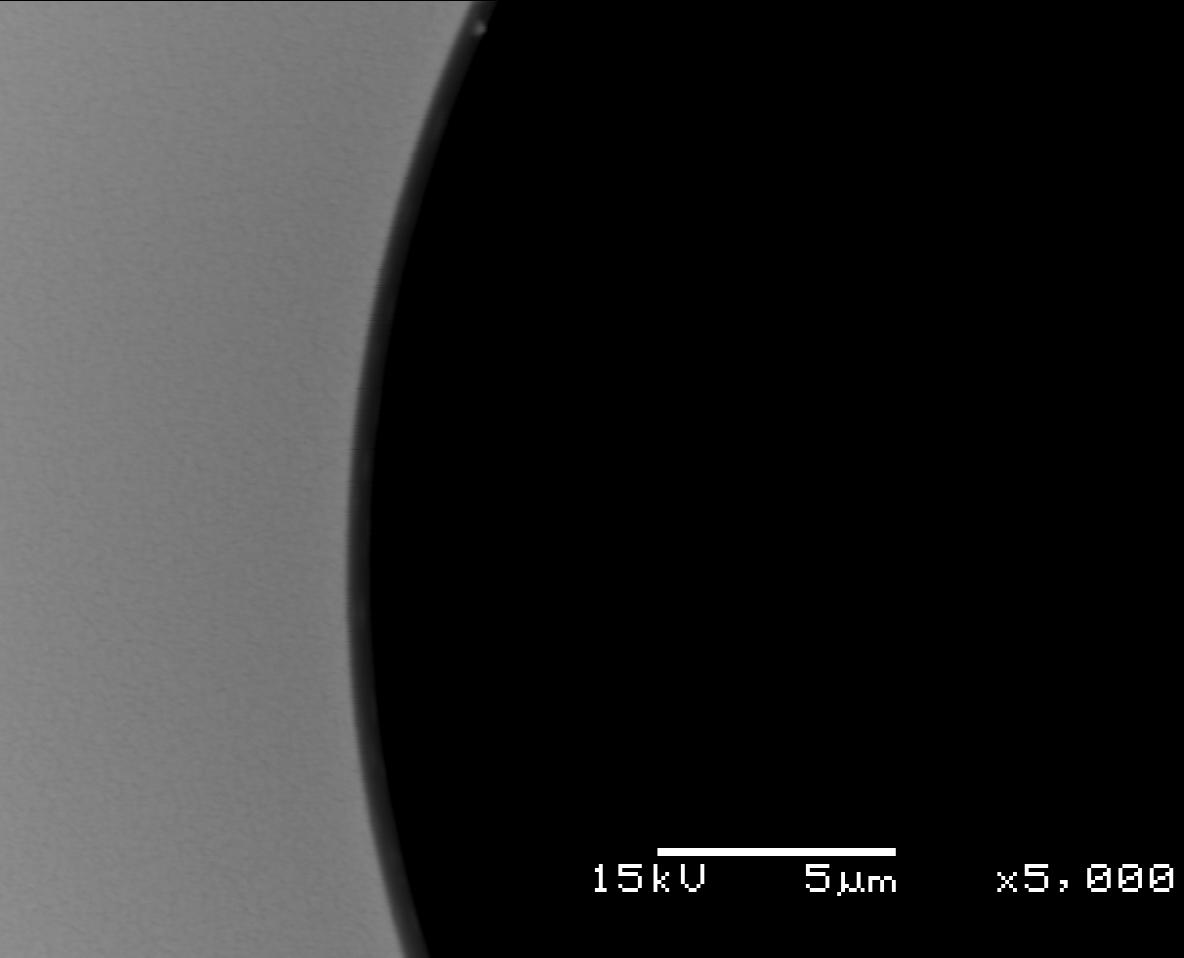
\includegraphics[width=0.8\textwidth,natwidth=4.17in,natheight=3.32in]{./Figures/A_003.pdf}
	\rule{35em}{0.5pt}
	\caption["Capillary wall"]{"A SEM image displaying the smoothness of a capillary wall."}
	\label{fig:TheFigureLabel}
\end{figure}


Since the orifices in these pictures are between 10 and 20 micron in diameter, we concluded that it was not material from the column that plugged the orifice. 

We observed one plugged restrictor with visible black material in the orifice that seemed to have been plugged by piece of stainless steel shaving. The elemental analysis suggest that the angular piece visible in the hole consisted of iron, chromium and nickel.

\begin{figure}[htbp]
	\centering
	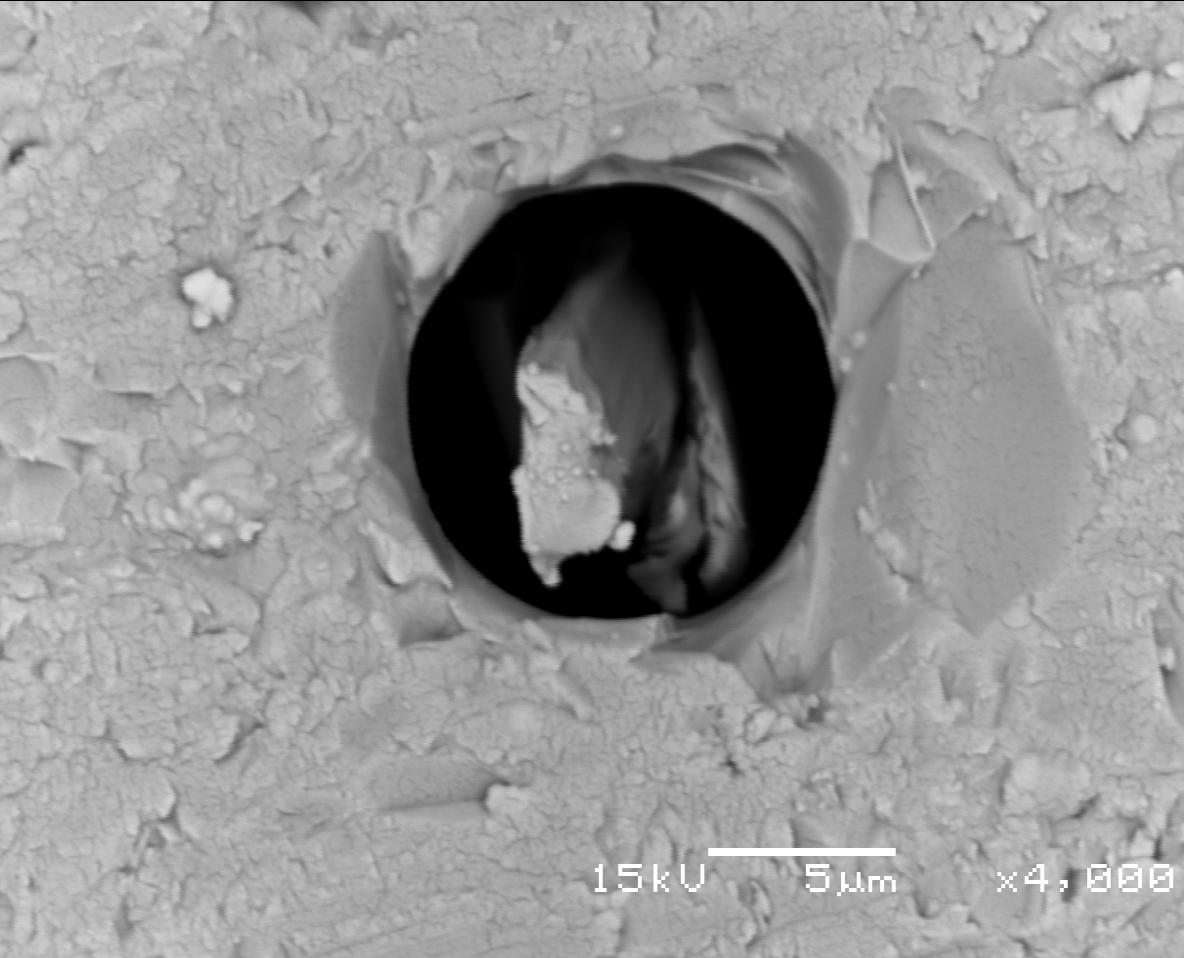
\includegraphics[width=0.8\textwidth,natwidth=4.17in,natheight=3.32in]{./Figures/H_004.pdf}
	\rule{35em}{0.5pt}
	\caption["A shaving-plugged orifice"]{"A SEM image of an orifice plugged by a shaving of stainless steel. "}
	\label{fig:H004}
\end{figure}


The plugging by colourless material, combined with the fact that plugging only appeared when the pressure in the restrictor cycled, we developed a hypothesis that the plugging was caused by material dissolved in the system which preciptated during the pressure cycle in the restrictor capillary.

This seems to be confirmed by the image of one restrictor covered by a smooth material, completely blocking the end face of the capillary.

\begin{figure}[htbp]
	\centering
	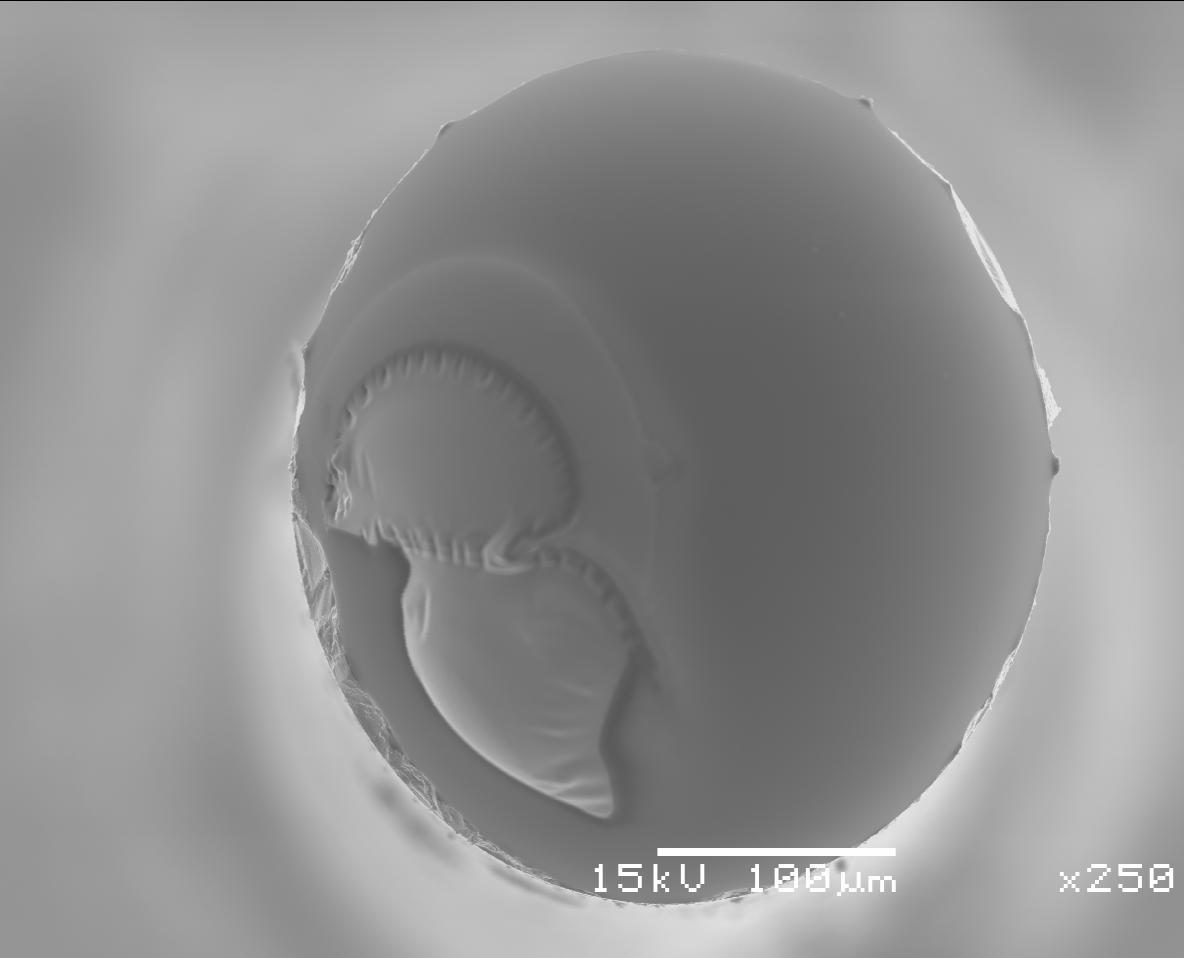
\includegraphics[width=0.8\textwidth,natwidth=4.17in,natheight=3.32in]{./Figures/F_001.pdf}
	\rule{35em}{0.5pt}
	\caption["A restrictor covered by a soft material"]{"A SEM image of an orifice completely plugged and the capillary end coated with a soft, smooth material."}
	\label{fig:F001}
\end{figure}

In addition, the inside of a capillary blocked with no visible material shows a deposit on the inside of the wall. 

\begin{figure}[htbp]
	\centering
	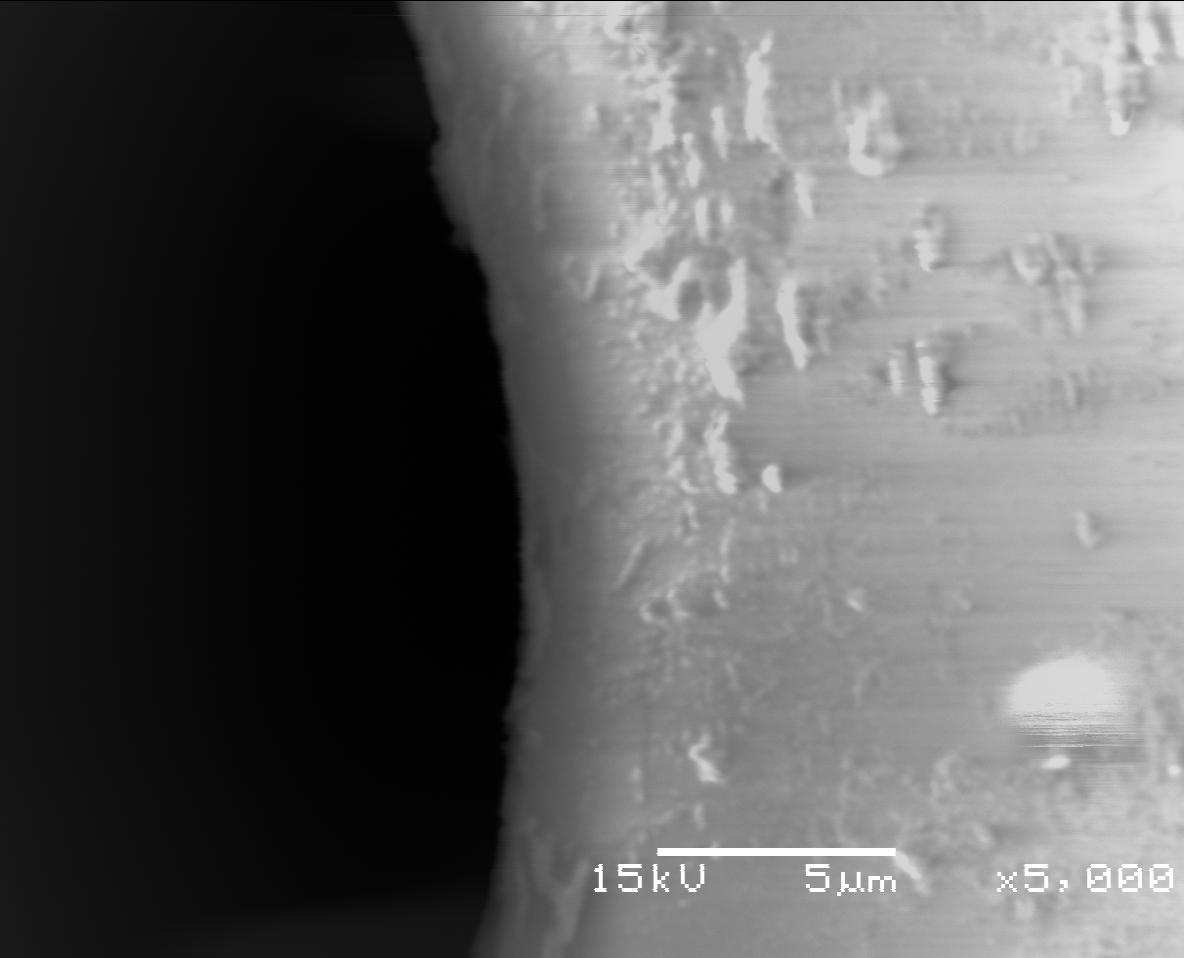
\includegraphics[width=0.8\textwidth,natwidth=4.17in,natheight=3.32in]{./Figures/D_004.pdf}
	\rule{35em}{0.5pt}
	\caption["A coating on the inside of a capillary"]{"A SEM image showing a layer precipitated on the inside wall a capillary."}
	\label{fig:D004}
\end{figure}

The smallness of the orifice contributes to the plugging problem. With a diameter of 50 $\mu$m, a solid sphere that fits in this capillary will have a volume of .065nL, or 65pL. This means that nanogram quantities of materail can easily block the restrictor. 

On re-examining our assumptions about the evaporation process, we saw the the evaporation process is not as strenuous as we thought, and the linear restrictor would probably be adequate. 

We therefore switched our restrictor choice to the linear restrictor. 1

\section{Detectors}

UV: CO2 transparency 

\section{Software} % Or should this be a separat Chapter?


The hardware described above were of course controlled by software. 

The controlling software was based on the graphical programming platform LabVIEW, version 7.11, supplied by National Instruments. This interfaced easily with the National Instruments PIC 512 E multi-IO card. 

\subsection{Instrument Control}
A number of individual PID controllers were used. The tuning of the PID controllers were done according to \cite{Peacock}.

Each controller uses an individual WHILE loop in LabVIEW. I discovered that apparently every WHILE loop runs in it's own thread, independently of the other loops in the VI, as long as there are no wires connecting two loops. In that case the loop will naturally pause until it gets data from all the wires, meaning that the running of the slower loop will determine the rate of execution of the other loop. 

The ``main loop'' in the program is the one that determines the state of the instrument.

To make sense of all the different settings in the instrument, the instrument had different `states'. The SFC had different states, and one of these states triggered and contained the states of the GC. 

The SFC had the following states:
\begin{description}
	\item[0. Idle] Pump off. Stop valve shut.
	\item[1. Equilibrate] Pump running. Stop valve open.
	\item[2. Loading] Sample valve on `Load'. GC at purge temperature. Stop valve shut.
	\item[3. Dead volume] Sample valve switches to `Inject'. Pump running. Stop valve open. 
	\item[4. Pre GC Time] Wait for dead volume time to pass.
	\item[5. Cryo] Cryo valve opens.
	\item[6. Cooling] GC column cools.
	\item[7. Collecting] Stop valve opens. 
	\item[8. Wait for GC\_sampled] Wait for collecting period.
	\item[9. Inlet flush] Stop valve shuts. Sample enters GC column. Inlet pressure rises.
	\item[10. Wait for sample to enter column]
	\item[11. Inlet vent] Inlet vent valve opens. Inlet pressure returns to normal.
	\item[12. Wait for inlet venting] Inlet vents and inlet is flushed with hydrogen.
	\item[13. GC Run] The inlet valve shuts. A GC run is started.
	\item[14. Wait for GC to finish]
	\item[15. End of GC run]
	\item[16. Emergency Stop or Initialise]
\end{description}

At the end of the GC run the state returns to `Cryo' (5), except if the set duration of the SFC run has been exceeded, in which case it switches to `Idle' (0).

The GC had the following states

\begin{description}
	\item[0. Idle] Nothing happens. GC temperature is set by an Idle Temperature control.
	\item[1. Start GC run] Toggles a flag that show that the temperature ramp is running.
	\item[2. Wait for equilibrium] Wait for the start temperature to be reached.
	\item[3. Start gradient] Set the ramp start time.
	\item[4. Run Gradient] Set temperature to current ramp temperature. Write data.
	\item[5. End Run] Write time at end of data strip. Return to `Idle' state. `
\end{description}



The coaxial heater had it's own loop to control the heating and cooling. The temperature setpoint was set by the GC ramp, via the GC `Run gradient' state.  

Each of the inlet leg and outlet leg heaters had it's own PID loop. The output of the PID loop was a percentage duty cycle used in the pulse-width modulation (PWM) of the power to the heater, implemented by switching the power to the heater on and off. This PWM had a very long period (5 seconds) , so it was adequate to implement it in software --- in industry they are more commonly implemented using hardware counter/timers. The power to the inlet and outlet leg heaters were switched on and off using solid state relays. These were easily controlled by the digital output controls of the 

The pumps had their own loop. It didn't have a PID controller. The pulses to the pump were merely switched off when the pressure exceeded the setpoint by a set amount, and switched on when it fell below the setpoint. 

\subsection{Data collection and analysis.}

Data was collected in a file using the following format:

\begin{tabular}{|l|l|l|l|}
\hline
No & Data Type & Value & Units \\
\hline
1 & Integer8 & ID & None \\
2 & Real64 & Time & s \\
3 & Real64 & TAmbient & K  \\
4 & Real64 & Ttc & K \\
5 & Real64 & Vb & V \\
6 & Real64 & dV & V \\
7 & Real64 & P1 & Pa \\
8 & Real64 & P2 & Pa \\
9 & Real64 & TInlet & K \\
10 & Real64 & TOutlet & K \\
11 & Real64 & Detector & V \\
12 & Real64 & TColumn & K \\
13 & Real64 & P1 Setpoint & Pa \\
14 & Real64 & P2 Setpoint & Pa \\
15 & Real64 & TInlet Setpoint & K \\
16 & Real64 & TOutlet Setpoint & K \\
17 & Real64 & TColumn Setpoint & K \\
\hline

\end{tabular}

The values TAmbient to Detector are digitized measurements. TColumn is calculated from Vb and dV by the calibration formula. P1 setpoint to TColumn Setpoint are the setpoints from the control system. Including the setpoints makes the data files larger, but it gives invaluable information on the quality of the controlled quantities, and can greatly assist {\it post hoc} debugging.

In this table TAmbient is the temperature measured by the thermistor used for cold junction compensation. Ttc is the temperature of a free thermocouple used for measuring temperatures in various places. Vb is the voltage of the current-measuring circuit, and dV is the voltage of the voltage-measuring circuit of the coaxial heater. P1 is the pressure measured by the first piston pump, and P2 is the pressure measured by the modifier pump. TInlet and Toutlet are the temperatures of the inlet and outlet leg heaters respectively. 

The �Time� meaning depends on the �ID�. 

\begin{tabular}{|l|l|l|}

\hline
ID & Time Value & Meaning \\
\hline
0 & 0 & File Created \\
1 & SFC\_Run\_Time � Interval & Time of start of GC run \\
2 & Current time � GC\_Time0 & Data point of GC run \\
3 & SFC\_Run\_Time/60000 & End of GC run? \\
4 & SFC\_Run\_Time & End of SFC run \\
\hline

\end{tabular}

Naturally most of the data points would have ID = 2, and the rest are just time stamps to identify the times of the start of the end of the runs. 

This data structure is simple but not particularly portable, as is evident by the following note given in the LabVIEW documenation:
\begin{quote}
Note: LabVIEW uses the big-endian format when handling and storing multi-byte data, even on the Windows (x86) platform. Little Endian was the choice for computers based on the Intel x86 processors, while Motorola processors (including the Macintosh computer, for which LabVIEW was first developed) used big-endian. Be aware that C and other Windows applications typically expect numeric data to be in little-endian form.
\end{quote}

Source: http://digital.ni.com/public.nsf/allkb/8224F2391418FDF6862568F00051D091

Therefore the data was converted into the ANDI (netCDF) format. This format can be read by the ChromaTOF software by LECO, giving us access to a well-developed tool for 2D data analysis.

The conversion was done it a two-step process, to avoid having to develop custom software for a poorly-defined data file with a structure that's still in development. Using Mathematica, the data was written from LabVIEW binary to a NCL text file, which was then converted to netCDF using the utility ncGen. This generated a properly-formatted netCDf file. 

